\documentclass[14pt]{beamer}
\usetheme{Warsaw}
\usecolortheme{beaver}
\usefonttheme{professionalfonts}

\input{../../preamble}
\usepackage{amscd,amsmath,amssymb,amsthm,graphicx}
\usepackage[mathscr]{eucal}
\usepackage{paralist}
\usepackage{tabto}
\usepackage[normalem]{ulem}

% % % % % % % % % %
\title[Cal I S2015]{MATH 2554 (Calculus I)}
\subtitle{}
\author[Wheeler]{Dr. Ashley K. Wheeler}
\institute{University of Arkansas}
\date{\today}
\logo{}

% % %
\begin{document}
\maketitle

% % %
\begin{frame}
\frametitle{Table of Contents}
\tableofcontents
\end{frame}

% % % % % % % % % % Mon 2 Feb 2015

% % %
\begin{frame}
\section[Week 4]{Week 4: 2-6 January}
\frametitle{Monday 2 February (Week 4)}
\begin{itemize}
\item EXAM \#1: Friday 6 February 
	\begin{itemize}
	\item in class
	\item covers up to and including $\oint 3.1$
	\end{itemize}
\end{itemize}
\end{frame}

% % %
\subsection[3.1 Introducing the Derivative]{$\oint$ 3.1 Introducing the Derivative}
% % %

% % %
\begin{frame}
\frametitle{$\oint$ 3.1 Introducing the Derivative}
\small
{\bf Recall from Ch 2:}  We said that the slope of the tangent line at a point is the limit of the slopes of the secant lines as the points get closer and closer.

\vspace{0.5pc}
\begin{itemize}
\item slope of secant line:  $\dfrac{f(x)-f(a)}{x-a}$\ (avg.\ rate of change) 

\vspace{0.5pc}
\item slope of tangent line:  $\displaystyle\lim_{x \to a} \frac{f(x)-f(a)}{x-a}$\ (instantaneous rate of change)
\end{itemize}
\end{frame}

% % %
\begin{frame}
\frametitle{}
\centering{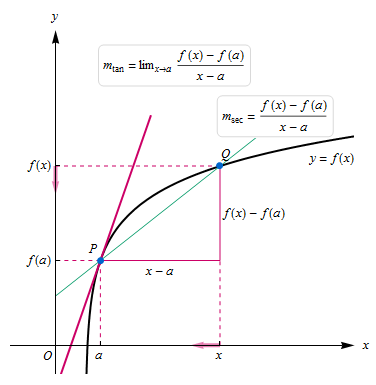
\includegraphics[scale=0.75]{lim}}
\end{frame}

% % %
\begin{frame}
\frametitle{Example}
Use the relationship between secant lines and tangent lines, specifically the slope of the tangent line, to find the equation of a line tangent to the curve $f(x)=x^2+2x+2$ at the point $P=(1,5)$.
\end{frame}

% % %
\begin{frame}
\frametitle{}
\small
In the preceding example, we considered two points 
\vspace{-0.5pc}
\[P=\left(a,f(a)\right)\quad\text{and}\quad Q=\left(x,f(x)\right)\]

\vspace{-0.5pc}
that were getting closer and closer together.

\vspace{3pc}
Instead of looking at the points approaching one another, we can also view this as the distance $h$ between the points approaching 0.  For 
\vspace{-0.5pc}
\[P=\left(a,f(a)\right)\quad\text{and}\quad Q=\left(a+h,f(a+h)\right),\]
\end{frame}

% % %
\begin{frame}
\footnotesize
\begin{itemize}
\item slope of secant line:  $\dfrac{f(a+h)-f(a)}{(a+h)-a}= \dfrac{f(a+h)-f(a)}{h}$

\vspace{1.5pc}
\item slope of tangent line:  $\displaystyle\lim_{h \to 0} \frac{f(a+h)-f(a)}{h}$
\end{itemize}
\end{frame}

% % %
\begin{frame}
\frametitle{}
\centering{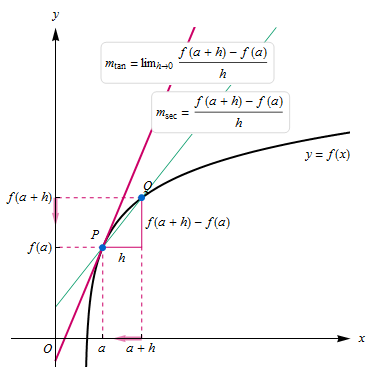
\includegraphics[scale=0.75]{limDef3_1}}
\end{frame}

% % %
\begin{frame}
\frametitle{Example}
Find the equation of a line tangent to the curve $f(x)=x^2+2x+2$ at the point $P=(2,10).$
\end{frame}

% % %
\begin{frame}
\frametitle{Derivative Defined as a Function}
\small
The slope of the tangent line for the function $f$ is a function of $x$, called the derivative of $f$.
\begin{dfn}
\footnotesize
The \emph{derivative} of $f$ is the function 
$$f^{\prime}(x)=\lim_{h \to 0} \frac{f(x+h)-f(x)}{h}$$
provided the limit exists.  If $f^{\prime}(x)$ exists, we say $f$ is \emph{differentiable} at $x$.  If $f$ is differentiable at every point of an open interval $I$, we say that $f$ is differentiable on $I$.
\end{dfn}
\end{frame}

% % %
\begin{frame}
\frametitle{}
Use the definition of the derivative to find the derivative of the function $f(x)=x^2+2x+2.$
\end{frame}

% % %
\begin{frame}
\frametitle{Leibniz Notation}
\small
A standard notation for change involves the Greek letter $\Delta$. 
\[\frac{f(a+h)-f(a)}{h}=\frac{f(x+\Delta x)}{\Delta x}=\frac{\Delta y}{\Delta x}.\]

\vspace{2pc}
Apply the limit:
\[f^{\prime}(x)=\lim_{\Delta x \to 0} \frac{f(x+\Delta x)}{\Delta x}=\lim_{\Delta x \to 0} \frac{\Delta y}{\Delta x}=\frac{dy}{dx}\]
\end{frame}

% % %
\begin{frame}
\frametitle{Other Notation}
\small
The following are alternative ways of writing $f^{\prime}(x)$ (i.e., the derivative as a function of $x$):
\[\frac{dy}{dx}\qquad\frac{df}{dx} \qquad\frac{d}{dx}\left(f(x)\right) \qquad D_x (f(x)) \qquad y^{\prime}(x)\]

\vspace{2pc}
The following are ways to notate the derivative of $f$ evaluated at $x=a$:
\[f^{\prime}(a)\qquad y^{\prime}(a) \qquad \left. \frac{df}{dx} \right|_{x=a} \qquad \left. \frac{dy}{dx} \right|_{x=a}\]
\end{frame}

% % %
\begin{frame}
\frametitle{Graphing the Derivative}
\small
The graph of the derivative is the graph of the collection of slopes of tangent lines of a graph.  If you just have a graph (without an equation for the graph), the best you can do is approximate the graph of the derivative.
\end{frame}

% % %
\begin{frame}
\frametitle{}
\footnotesize
Simple checklist:
\begin{itemize}
\item[1.] Note where $f^{\prime}(x)=0$.
\item[2.]  Note where $f^{\prime}(x)>0$.  (What does this look like?)
\item[3.]  Note where $f^{\prime}(x)<0$.  (What does this look like?)
\end{itemize}
\centering{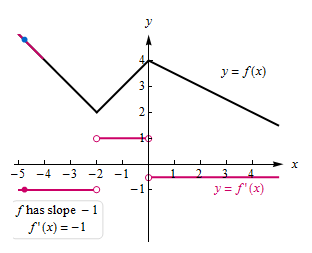
\includegraphics[scale=0.7]{graphDeriv3_1}}
\end{frame}

% % %
\begin{frame}
\frametitle{Differentiability vs. Continuity}
\small
Key points about the relationship between differentiability and continuity:

\begin{itemize}
\item If $f$ is differentiable at $a$, then $f$ is continuous at $a$.
\item If $f$ is not continuous at $a$, then $f$ is not differentiable at $a$.
\item $f$ can be continuous at $a$, but not differentiable at $a$.
\end{itemize}
\end{frame}

% % %
\begin{frame}
\frametitle{}
\small
A function $f$ is \underline{not} differentiable at $a$ if at least one of the following conditions holds:
\begin{itemize}
\item[1.] $f$ is not continuous at $a$.
\item[2.] $f$ has a corner at $a$.  (Why does this make $f$ not differentiable?)
\item[3.] $f$ has a vertical tangent at $a$.  (Why does this make $f$ not differentiable?)
\end{itemize}
\end{frame}

% % %
\begin{frame}
\frametitle{HW from Section 3.1}  
Do problems 11--12, 19--20, 23--26, 31--33, 35--36, 39--43, 45, 49--52 (pp.\ 131--133 in textbook)

\bigskip
{\bf NOTE:}  You do not know any rules for differentiation yet (e.g., Power Rule, Chain Rule, etc.)  In this section, you are strictly using the definition of the derivative and the definition of slope of tangent lines we have derived.
\end{frame}

% % % % % % % % % % Wed 4 Feb 2015

% % %
\begin{frame}
\frametitle{Wednesday 4 February (Week 4)}
\begin{itemize}
\item No quiz this week.

\vspace{0.5pc}
\item 2 quizzes next week:
	\begin{itemize}
	\item Tues 10 Feb in-drill group quiz (Quiz 4)
	\item Thurs 12 Feb usual weekly take-home quiz (Quiz 5)
	\end{itemize}
	
\vspace{0.5pc}
\item EXAM \#1: Friday 6 February 
	\begin{itemize}
	\item in class
	\item covers up to and including $\oint 3.1$
	\item one $3\times 5$ inch notecard, one-sided only, allowed
	\item only the approved calculator allowed (see syllabus)
	\end{itemize}
\end{itemize}
\end{frame}

% % %
\subsection{Exam \#1 Review}
% % %

\begin{frame}
\frametitle{Exam \#1 Review}
\begin{itemize}
\item $\oint 2.1$  The Idea of Limits
	\begin{itemize}
	\item Understand the relationship between average velocity \& instantaneous velocity, and secant and tangent lines
	%\item Be able to compute average velocities and use the idea of a limit to approximate instantaneous velocities
	\item Be able to compute slopes of secant lines and use the idea of a limit to approximate the slope of the tangent line
	\end{itemize}
\item $\oint 2.2$ Definitions of Limits
	\begin{itemize}
	\item Know the definition of a limit
	%\item Be able to use a graph of a table to determine a limit
	\item Know the relationship between one- and two-sided limits
	\end{itemize}
\end{itemize}
\end{frame}

% % %
\begin{frame}
\begin{itemize}
\item $\oint 2.3$ Techniques for Computing Limits
	\begin{itemize}
	\item Know and be able to compute limits using analytical methods (e.g., limit laws, additional techniques)
	\item Know the Squeeze Theorem and be able to use it to determine limits
	\end{itemize}
	
\vspace{1pc}
\begin{ex} Evaluate $\displaystyle\lim_{x\to 0}x\sin{\frac{1}{x}}$. \end{ex}	
\end{itemize}	
\end{frame}

% % % 
\begin{frame}
\begin{itemize}
\item $\oint 2.4$ Infinite Limits
	\begin{itemize}
	%\item Be able to use a graph, a table, or analytical methods to determine infinite limits
	\item Know the definition of a vertical asymptote  and be able to determine whether a function has vertical asymptotes 
	\end{itemize}
\item $\oint 2.5$ Limits at Infinity
	\begin{itemize}
	\item Be able to find limits at infinity and horizontal asymptotes 
	\item Know how to compute the limits at infinity of rational functions
	\end{itemize}
\end{itemize}
\end{frame}

% % %
\begin{frame}
\frametitle{}
\begin{ex} Determine the end behavior of $f(x)$.  If there is a horizontal asymptote, then say so.  Next, identify any vertical asymptotes.  If $x=a$ is a vertical asymptote, then evaluate $\displaystyle\lim_{x\to a^+}f(x)$ and $\displaystyle\lim_{x\to a^-}f(x)$.
\[f(x)=\frac{2x^3+10x^2+12x}{x^3+2x^2}\]
\end{ex}
\end{frame}

% % %
\begin{frame}
\begin{itemize}
\item $\oint 2.6$ Continuity 
	\begin{itemize}
	\item Know the definition of continuity and be able to apply the continuity checklist
	\item Be able to determine the continuity of a function (including those with roots) on an interval
	\item Be able to apply the Intermediate Value Theorem to a function
	\end{itemize}
\end{itemize}
\end{frame}

% % %
\begin{frame}
\frametitle{}
\begin{ex} Determine the value for $a$ that will make $f(x)$ continuous. 
\[f(x)=\begin{cases}
	\frac{x^2+3x+2}{x+1} & x\neq -1 \\
	a & x=-1
	\end{cases}\]
\end{ex}
\end{frame}

% % %
\begin{frame}
\frametitle{}
\begin{ex} Show that $f(x)=2$ has a solution on the interval $(-1,1)$, with
\[f(x)=2x^3+x.\]
\end{ex}
\end{frame}

% % %
\begin{frame}
\begin{itemize}
\item $\oint 2.7$ Precise Definition of Limits 
	\begin{itemize}
	\item Understand the $\delta$, $\epsilon$ relationship for limits
	\item Be able to use a graph or analytical methods to find a value for $\delta>0$ given an $\epsilon>0$ (including finding symmetric intervals)
	\end{itemize}
\end{itemize}
\end{frame}

% % %
\begin{frame}
\frametitle{}
\footnotesize
In this example, the two-sided limits at $x=1$ and $x=2$ do not exist.
\begin{columns}[T]
\begin{column}{.5\textwidth}
\begin{block}
\centering{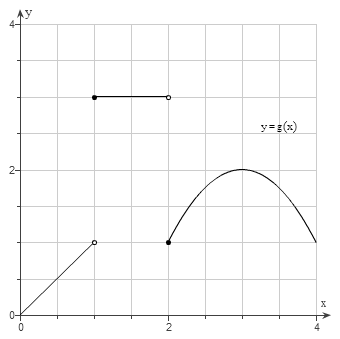
\includegraphics[scale=0.6]{Exam1pic}}
\end{block}
\end{column}
\begin{column}{.5\textwidth}
\begin{block}
{Example}
\footnotesize
Use the graph to find the appropriate $\delta$.
\begin{itemize}
\item[(a)] $|g(x)-2|<\frac{1}{2}$ whenever $0<|x-3|<\delta$

\vspace{0.5pc}
\item[(b)] $|g(x)-1|<\frac{3}{2}$ whenever $0<|x-2|<\delta$
\end{itemize}
\end{block}
\end{column}
\end{columns}
\end{frame}

% % %
\begin{frame}
\begin{itemize}
\item $\oint 3.1$ Introducing the Derivative
	\begin{itemize}
	\item Know the definition of a derivative and be able to use this definition to calculate the derivative of a given function
	\item Be able to determine the equation of a line tangent to the graph of a function at a given point
	\item Know the 3 conditions for when a function is not differentiable at a point, and why these three conditions make a function not differentiable at the given point
	\end{itemize}
\end{itemize}
\end{frame}

% % %
\begin{frame}
\begin{ex}
	\begin{itemize}
	\item[(a)] Use the limit definition of the derivative to find an equation for the line tangent to $f(x)$ at $a$, where
	\[f(x)=\frac{1}{x};\qquad a=-5.\]
	
	\vspace{0.5pc}
	\item[(b)] Using the same $f(x)$ from part (a), find a formula for $f'(x)$ (using the limit definition).
	
	\vspace{0.5pc}
	\item[(c)] Plug $-5$ into your answer for (b) and make sure it matches your answer for (a).
	\end{itemize}
\end{ex}
\end{frame}

% % %
\begin{frame}
\frametitle{Other Study Tips}
\footnotesize
\begin{itemize}
\item Brush up on algebra, especially radicals.
\item If your answer is something like $\sqrt 2$, don't plug that into your calculator, just leave it as is.
\item When in doubt, show steps.  See the document camera notes to get an idea of what's expected.
\item You will be punished for wrong notation; e.g., the limit symbol.
\item Read the question!  Several students always lose points because they didn't answer the question or they didn't follow directions.
\item Do the book problems.
\item Look at the pictures in the book and the interactive applets on MLP.
\end{itemize}
\end{frame}


\begin{comment}
\end{comment}

\end{document}